\section{Work Environment Example}
The following is a deployment example of the system that has been previously described.
TODO: esempio di deployment con immagine casa.

\begin{figure}[H]
	\begin{center}
		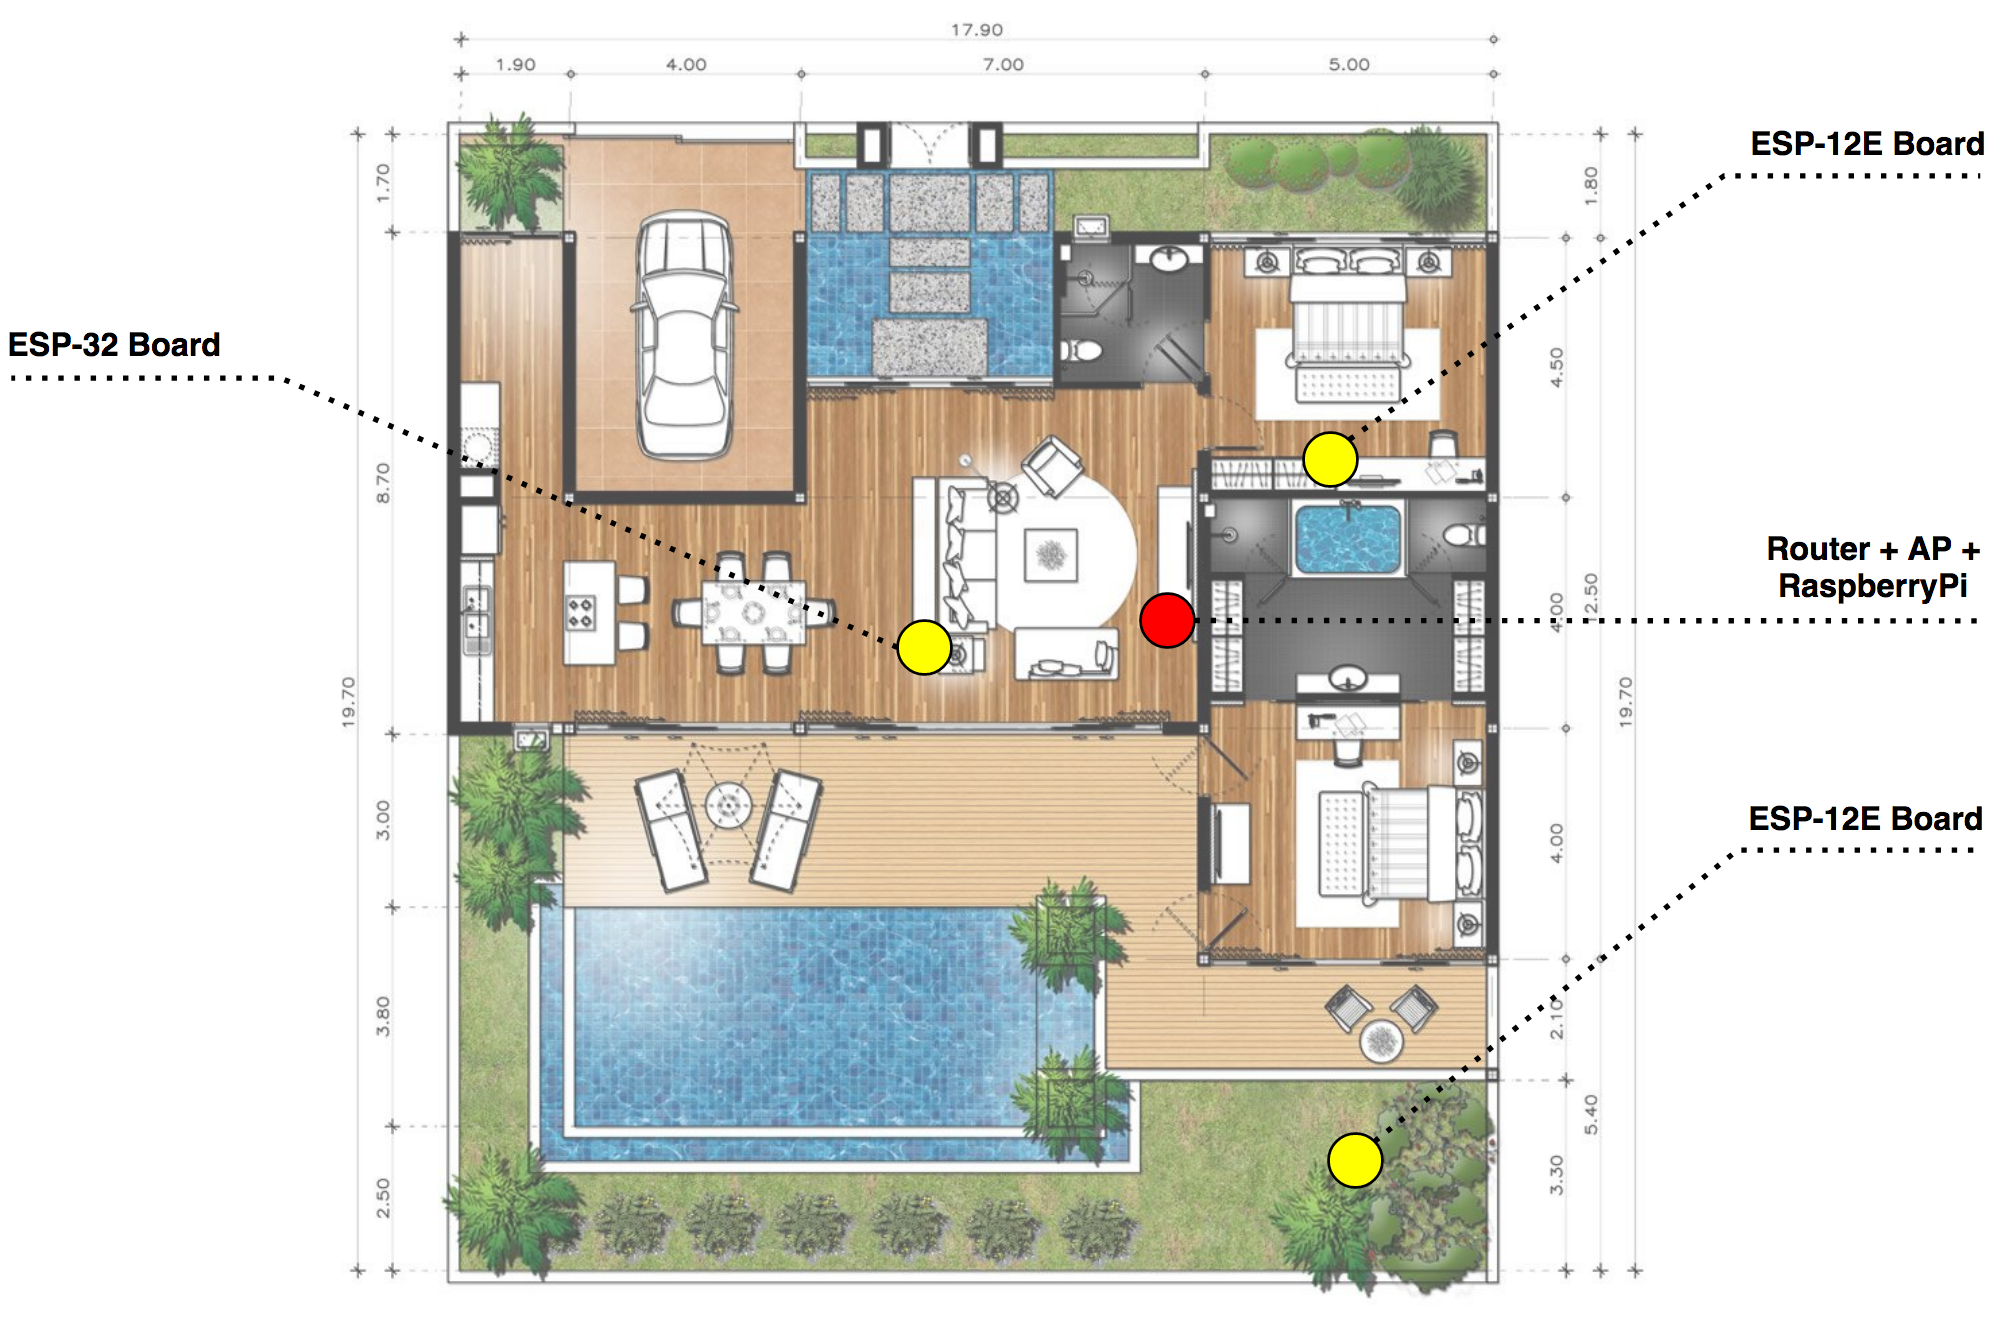
\includegraphics[width=\textwidth]{./pictures/blueprint_deployment.png}
		\caption{Blueprint of a typical house showing the position of all the system nodes.}
		\label{blueprint_deployment}
	\end{center}
\end{figure}

\section{Future Extensions}
The system implementation opens the possibility of including new features. For example:

\begin{itemize}
	\item The possibility of adding more boards to cover larger areas and collect more information about the surrounding environment;
	\item The possibility of using different sensors in addition to the simple temperature, humidity and light ones of the current implementation.
	\item The possibility of using \textit{energy harvesting} to derive energy from external sources, such as solar power and wind energy.
\end{itemize}